\documentclass[11pt]{article}
\usepackage[margin=1in]{geometry}
\usepackage{amsmath,amssymb,amsthm,mathtools}
\usepackage{microtype}
\usepackage[hidelinks]{hyperref}
\usepackage{tikz}
\usetikzlibrary{patterns}

\newtheorem{theorem}{Theorem}
\newtheorem{proposition}[theorem]{Proposition}
\newtheorem{lemma}[theorem]{Lemma}
\newtheorem{corollary}[theorem]{Corollary}
\theoremstyle{definition}
\newtheorem{definition}[theorem]{Definition}
\newtheorem{example}[theorem]{Example}
\theoremstyle{remark}
\newtheorem{remark}[theorem]{Remark}

\newcommand{\R}{\mathbb{R}}
\newcommand{\eps}{\varepsilon}
\newcommand{\Bx}{\mathcal{B}}
\newcommand{\Reach}{\mathcal{R}}
\newcommand{\abs}[1]{\left\lvert #1 \right\rvert}
\newcommand{\norm}[1]{\left\lVert #1 \right\rVert}

\title{Joint Tracking of Correlated Quantities in Cert-RNN+:\\ Mathematical Formulation}
\author{Cert-RNN+ benchmark notes}
\date{9 October 2026}

\begin{document}
\maketitle

\begin{abstract}
Cert-RNN+ certifies that an LSTM-autoencoder anomaly detector raises no false alarm for any input in a perturbation box. It is built on the zonotope (affine-arithmetic) abstract domain, in which every intermediate quantity is an affine function of a shared vector of noise symbols. This note states the soundness invariant of that domain and derives the two refinements that distinguish Cert-RNN+ from Cert-RNN: (i) \emph{linked gates}, which bound each bilinear gate product over the joint reachable region of its two operands instead of over their bounding box, and (ii) a \emph{joint score bound}, which bounds the reconstruction error of all outputs together instead of component by component. Both refinements are sound and never looser than the baseline. We also explain why box-based linear relaxations, as used by CROWN, cannot exploit the same structure.
\end{abstract}

\section{Setting}

\paragraph{Detector.} An LSTM autoencoder maps a window $x \in \R^{T\times D}$ ($T$ seconds, $D$ features) to a reconstruction $\hat x = \mathrm{AE}(x)$. The encoder LSTM produces one code per second; the decoder LSTM reads the code of second $t$ at step $t$, followed by a linear head. The anomaly score is the mean squared reconstruction error
\begin{equation}
s(x) \;=\; \frac{1}{N}\norm{\mathrm{AE}(x) - x}_2^2, \qquad N = TD,
\label{eq:score}
\end{equation}
and an alarm is raised iff $s(x) > \tau$, where $\tau$ is a threshold fixed from validation data.

\paragraph{LSTM step.} With pre-activations $a^{(\cdot)} = W^{(\cdot)} x_t + U^{(\cdot)} h_{t-1} + b^{(\cdot)}$, one step is
\begin{equation}
i_t = \sigma(a^{(i)}),\; f_t = \sigma(a^{(f)}),\; g_t = \tanh(a^{(g)}),\; o_t = \sigma(a^{(o)}),\quad
c_t = f_t \odot c_{t-1} + i_t \odot g_t,\quad h_t = o_t \odot \tanh(c_t).
\label{eq:lstm}
\end{equation}
The non-linear operations are therefore of two kinds: unary activations ($\sigma$, $\tanh$) and \emph{bilinear products of correlated operands}: $\sigma(\cdot)\cdot\tanh(\cdot)$ (in $i_t\odot g_t$ and $o_t\odot\tanh(c_t)$) and $\sigma(\cdot)\cdot(\cdot)$ (in $f_t\odot c_{t-1}$).

\paragraph{Property (no false alarm).} Let $x^0$ be a normal window with $s(x^0)\le\tau$, let $F \subseteq \{1,\dots,T\}$ be the attacked seconds, and let $\epsilon>0$. The perturbation set is
\begin{equation}
X_\epsilon = \bigl\{\, x : \abs{x_{t,d} - x^0_{t,d}} \le \epsilon \text{ for } t\in F,\ x_{t,d} = x^0_{t,d} \text{ for } t\notin F \,\bigr\}.
\end{equation}
The property is $\forall x\in X_\epsilon:\ s(x)\le\tau$. A verifier proves it by computing a sound upper bound $\bar s \ge \max_{x\in X_\epsilon} s(x)$ and checking $\bar s \le \tau$.

\section{Zonotopes and affine forms}

\begin{definition}[Affine form, zonotope]
Fix a vector of noise symbols $\eps\in[-1,1]^p$. An \emph{affine form} is $\hat z = c + g^\top \eps$ with $c\in\R$, $g\in\R^p$. A vector of $n$ affine forms sharing the same symbols, $\hat z = c + G\eps$ with $G\in\R^{n\times p}$, denotes the \emph{zonotope}
\begin{equation}
Z(c,G) = \{\, c + G\eps : \eps\in[-1,1]^p \,\} \subseteq \R^n .
\end{equation}
\end{definition}

Geometrically, $Z(c,G)$ is the Minkowski sum of the $p$ segments $[-G_{:,j}, G_{:,j}]$, translated by $c$; it is a centrally symmetric convex polytope \cite{ziegler1995}. The interval hull (bounding box) of coordinate $k$ is $[c_k - \norm{G_{k,:}}_1,\ c_k + \norm{G_{k,:}}_1]$.

\paragraph{Input encoding.} Assign one symbol to every attacked reading. Then $X_\epsilon = Z(x^0, G_0)$ exactly, where $G_0$ has entry $\epsilon$ in the row of reading $(t,d)$ and the column of its symbol, and zeros elsewhere. Every quantity computed from the input is subsequently expressed over the \emph{same} symbols, plus fresh symbols introduced by non-linear steps.

\paragraph{The soundness invariant.} Abstract interpretation \cite{cousot1977} with affine arithmetic \cite{comba1993,defigueiredo2004} maintains:

\begin{quote}
\textbf{(I)} For every concrete input $x\in X_\epsilon$ there exists an assignment $\eps\in[-1,1]^p$ of \emph{all} symbols (input and fresh) such that every tracked quantity equals the value of its affine form at $\eps$.
\end{quote}

Invariant (I) is what allows several quantities to be reasoned about \emph{jointly}: a single assignment $\eps$ is one concrete scenario, and every affine form is evaluated in that same scenario. Two forms that share symbols are therefore correlated, and the correlation is exact. Zonotope analyses of neural networks build on this \cite{ghorbal2009,gehr2018,singh2018}, including Cert-RNN for recurrent networks \cite{du2021}.

\begin{proposition}[Affine operations are exact]
If $\hat z = c + G\eps$ satisfies (I), so does $W\hat z + b = (Wc + b) + (WG)\eps$, with no approximation.
\end{proposition}
\begin{proof}
For the assignment $\eps$ given by (I), $Wz + b = W(c+G\eps) + b$.
\end{proof}

\begin{proposition}[Unary non-linearities]
Let $\hat z = c + g^\top\eps$ satisfy (I), with interval hull $[l,u]$, and let $\phi\in\{\sigma,\tanh\}$. Choose $a, b\in\R$ and $\beta \ge \max_{z\in[l,u]}\abs{\phi(z) - (az+b)}$. Then
\begin{equation}
\widehat{\phi(z)} = a\hat z + b + \beta\,\eps_{\mathrm{new}}
\end{equation}
with a fresh symbol $\eps_{\mathrm{new}}\in[-1,1]$ satisfies (I).
\end{proposition}
\begin{proof}
For the concrete value $z\in[l,u]$, set $\eps_{\mathrm{new}} = (\phi(z) - az - b)/\beta \in [-1,1]$ (any value if $\beta = 0$).
\end{proof}

\begin{remark}
The term $a\hat z$ keeps all symbols of $\hat z$, so the output stays correlated with every other quantity that shares them; only the error part $\beta\eps_{\mathrm{new}}$ is independent. Cert-RNN's specific choices of $(a,b,\beta)$ \cite{du2021} are used unchanged; the refinements below concern only bilinear products and the score.
\end{remark}

\section{The joint reachable region of two correlated quantities}

Consider two tracked quantities that share symbols,
\begin{equation}
\begin{pmatrix} \hat x\\ \hat y\end{pmatrix} = \begin{pmatrix} c_x\\ c_y\end{pmatrix} + \begin{pmatrix} g_x^\top\\ g_y^\top\end{pmatrix}\eps,\qquad \eps\in[-1,1]^p .
\end{equation}

\begin{lemma}[Joint region is a zonogon]
The set of pairs reachable under (I), $Z_{xy} = \{(c_x + g_x^\top\eps,\ c_y + g_y^\top\eps) : \eps\in[-1,1]^p\}$, is the image of the cube $[-1,1]^p$ under a linear map $\R^p\to\R^2$: a centrally symmetric convex polygon with at most $2p$ edges (a \emph{zonogon}). It satisfies
\begin{equation}
Z_{xy} \subseteq \Bx_{xy} \coloneqq [c_x \pm \norm{g_x}_1] \times [c_y \pm \norm{g_y}_1],
\end{equation}
and a corner of $\Bx_{xy}$ belongs to $Z_{xy}$ only if a single $\eps$ attains both coordinate extremes, i.e.\ only if $\operatorname{sign}(g_{x,j})$ and $\operatorname{sign}(g_{y,j})$ agree (or disagree) consistently over all $j$ with $g_{x,j}g_{y,j}\neq 0$. Its area is
\begin{equation}
\operatorname{area}(Z_{xy}) = 4\sum_{1\le i<j\le p} \abs{\det\begin{pmatrix} g_{x,i} & g_{x,j}\\ g_{y,i} & g_{y,j}\end{pmatrix}} .
\label{eq:area}
\end{equation}
\end{lemma}
\begin{proof}
The image of a cube under a linear map is a zonotope; in $\R^2$ it is a polygon whose edges are the generator vectors $(g_{x,j}, g_{y,j})$, each used twice, sorted by angle, which gives at most $2p$ edges and central symmetry. The upper-right corner $(c_x+\norm{g_x}_1, c_y+\norm{g_y}_1)$ requires $\eps_j = \operatorname{sign}(g_{x,j})$ and $\eps_j = \operatorname{sign}(g_{y,j})$ for every $j$, which is possible only if the signs agree wherever both are non-zero; the other corners are analogous. Formula \eqref{eq:area} is the area of a Minkowski sum of the segments $[-v_j, v_j]$ with $v_j = (g_{x,j}, g_{y,j})$: each pair of segments contributes a parallelogram of area $\abs{\det(2v_i, 2v_j)} = 4\abs{\det(v_i,v_j)}$.
\end{proof}

\begin{example}
Let $\hat x = \eps_1 + \eps_2$ and $\hat y = \eps_1 - \eps_2$. Each ranges over $[-2,2]$, so $\Bx_{xy} = [-2,2]^2$ with area $16$. But $x = 2$ forces $\eps_1 = \eps_2 = 1$ and hence $y = 0$. The joint region is the diamond with vertices $(\pm2,0)$ and $(0,\pm2)$, of area $8$ by \eqref{eq:area}; none of the four box corners is reachable.
\begin{center}
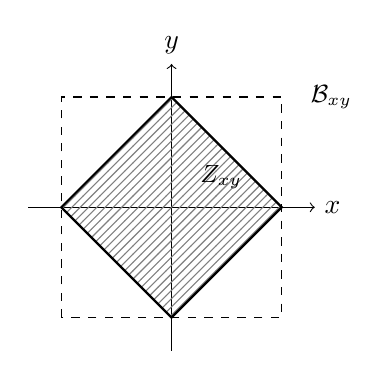
\begin{tikzpicture}[scale=0.7]
\draw[->] (-2.6,0) -- (2.6,0) node[right] {$x$};
\draw[->] (0,-2.6) -- (0,2.6) node[above] {$y$};
\draw[dashed] (-2,-2) rectangle (2,2);
\fill[pattern=north east lines, pattern color=gray] (2,0) -- (0,2) -- (-2,0) -- (0,-2) -- cycle;
\draw[thick] (2,0) -- (0,2) -- (-2,0) -- (0,-2) -- cycle;
\node at (2.9,2.0) {\small $\Bx_{xy}$};
\node at (0.9,0.55) {\small $Z_{xy}$};
\end{tikzpicture}
\end{center}
\end{example}

In an LSTM, the two operands of every gate product are computed from the same inputs and the same previous state, so they share many symbols and $Z_{xy}$ is typically a thin slanted polygon well inside $\Bx_{xy}$.

\section{Linked gates: bilinear products over the joint region}

Let $f(x,y)$ be one of the bilinear products in \eqref{eq:lstm}, $f = \sigma(x)\tanh(y)$ or $f = \sigma(x)\,y$, applied coordinate-wise to operands $(\hat x,\hat y)$.

\begin{definition}[Plane relaxation over a region]
For slopes $A, B\in\R$ (chosen as in Cert-RNN \cite{du2021}) and a set $S\subseteq\R^2$, let
\begin{equation}
C_1(S) = \inf_{(x,y)\in S}\bigl(f(x,y) - Ax - By\bigr),\qquad C_2(S) = \sup_{(x,y)\in S}\bigl(f(x,y) - Ax - By\bigr).
\end{equation}
\end{definition}

\begin{proposition}[Soundness of a plane relaxation]
If $S \supseteq Z_{xy}$, then
\begin{equation}
\widehat{f(x,y)} = A\hat x + B\hat y + \frac{C_1(S)+C_2(S)}{2} + \frac{C_2(S)-C_1(S)}{2}\,\eps_{\mathrm{new}}
\label{eq:bilinear}
\end{equation}
with a fresh symbol $\eps_{\mathrm{new}}\in[-1,1]$ satisfies (I).
\end{proposition}
\begin{proof}
Under (I), the concrete pair $(x,y)$ lies in $Z_{xy}\subseteq S$, so $C_1(S) \le f(x,y) - Ax - By \le C_2(S)$; choose $\eps_{\mathrm{new}}$ accordingly.
\end{proof}

The width $C_2(S) - C_1(S)$ is the new, uncorrelated error that enters the cell state $c_t$ and is carried to all later steps. Cert-RNN uses $S = \Bx_{xy}$. Cert-RNN+ uses a set between $Z_{xy}$ and $\Bx_{xy}$:

\begin{definition}[Grid cover]
Partition $\Bx_{xy}$ into an $n\times n$ grid of axis-aligned cells $Q_{1},\dots,Q_{n^2}$ and keep the cells that intersect the zonogon: $\mathcal{A} = \{Q_k : Q_k\cap Z_{xy}\neq\emptyset\}$. Set $S_+ = \bigcup_{Q\in\mathcal{A}} Q$. Then
\begin{equation}
C_1(S_+) = \min_{Q\in\mathcal{A}} C_1(Q),\qquad C_2(S_+) = \max_{Q\in\mathcal{A}} C_2(Q),
\end{equation}
where each $C_i(Q)$ is the exact extremum of $f - Ax - By$ over a box, computed by the same closed-form box enumeration Cert-RNN uses for $\Bx_{xy}$.
\end{definition}

\begin{theorem}[Linked gates are sound and never looser]
\label{thm:gates}
\begin{equation}
Z_{xy}\ \subseteq\ S_+\ \subseteq\ \Bx_{xy},
\end{equation}
hence \eqref{eq:bilinear} with $S = S_+$ satisfies (I), and
\begin{equation}
C_1(S_+) \ge C_1(\Bx_{xy}),\qquad C_2(S_+) \le C_2(\Bx_{xy}),\qquad C_2(S_+) - C_1(S_+) \le C_2(\Bx_{xy}) - C_1(\Bx_{xy}).
\end{equation}
\end{theorem}
\begin{proof}
Every point of $Z_{xy}\subseteq\Bx_{xy}$ lies in some cell, and that cell intersects $Z_{xy}$, so it is in $\mathcal{A}$; hence $Z_{xy}\subseteq S_+$. Each cell is a subset of $\Bx_{xy}$, hence $S_+\subseteq\Bx_{xy}$. Soundness follows from the previous proposition. An infimum over a subset is at least the infimum over the superset, and a supremum over a subset is at most the supremum over the superset.
\end{proof}

\paragraph{Deciding cell admission exactly.} A cell $Q$ (a rectangle) and $Z_{xy}$ (a convex polygon) are disjoint iff some axis separates them; by the separating-axis theorem for convex polygons it suffices to test the two coordinate axes and the edge normals of $Z_{xy}$, i.e.\ the normals of the generator vectors \cite{gottschalk1996,ericson2004}. The support of $Z_{xy}$ along a direction $w$ is $w^\top(c_x,c_y) \pm \sum_j \abs{w^\top(g_{x,j},g_{y,j})}$, computed exactly from all generators; the implementation adds a small outward tolerance, which can only admit more cells and therefore preserves soundness.

\paragraph{Two shortcuts that preserve soundness.}
\begin{enumerate}
\item \emph{Area-ratio skip.} If $\operatorname{area}(Z_{xy})/\operatorname{area}(\Bx_{xy}) > 0.9$, computed in closed form by \eqref{eq:area} before any cell is built, the zonogon nearly fills its box and the cover can recover little; the box result $S = \Bx_{xy}$ is used. This is sound because the box result is always sound, and it trades only tightness for time.
\item \emph{All-cells equality.} If every cell is admitted, $\mathcal{A}$ is the whole grid and $S_+ = \Bx_{xy}$; then $C_i(S_+) = C_i(\Bx_{xy})$ exactly, so the box result is returned without loss.
\end{enumerate}

\paragraph{Grid resolution.} The implementation uses $n = 16$ per axis. It was chosen in a development measurement (on models separate from the benchmark) of the fraction of the exact box-to-zonogon improvement recovered: $0.62$--$0.69$ at $n=8$, $0.80$--$0.85$ at $n=16$ and $0.89$--$0.93$ at $n=32$ for single-second perturbations, with cost roughly proportional to the number of admitted cells.

\section{Joint score bound}

After propagating all $T$ steps, the residuals $r = \mathrm{AE}(x) - x \in \R^N$ are affine in the \emph{same} symbol vector $\alpha\in[-1,1]^P$ (input symbols and all fresh symbols):
\begin{equation}
\hat r = c + V\alpha,\qquad c\in\R^N,\ V\in\R^{N\times P}.
\end{equation}
By (I) and \eqref{eq:score}, $\max_{x\in X_\epsilon} s(x) \le \frac1N\max_{\alpha\in[-1,1]^P}\norm{c+V\alpha}_2^2$.

\paragraph{Componentwise bound (Cert-RNN).}
\begin{equation}
\bar s_{\mathrm{comp}} = \frac1N\sum_{k=1}^{N}\bigl(\abs{c_k} + \norm{V_{k,:}}_1\bigr)^2 .
\label{eq:comp}
\end{equation}
Each term is the worst case of one residual, attained at its own $\alpha$; the sum lets every residual use a different $\alpha$, which cannot happen because there is only one.

\begin{theorem}[Joint score bound]
\label{thm:score}
\begin{equation}
\max_{\alpha\in[-1,1]^P}\norm{c+V\alpha}_2^2 \ \le\ \norm{c}_2^2 + 2\norm{V^\top c}_1 + \sum_{i,j=1}^{P}\abs{(V^\top V)_{ij}} \;\eqqcolon\; N\,\bar s_{\mathrm{joint}},
\label{eq:joint}
\end{equation}
and $\bar s_{\mathrm{joint}} \le \bar s_{\mathrm{comp}}$.
\end{theorem}
\begin{proof}
Expand $\norm{c+V\alpha}_2^2 = \norm{c}_2^2 + 2(V^\top c)^\top\alpha + \alpha^\top(V^\top V)\alpha$. With $\abs{\alpha_i}\le 1$: $(V^\top c)^\top\alpha \le \sum_i \abs{(V^\top c)_i}$ and $\alpha^\top M\alpha = \sum_{i,j} M_{ij}\alpha_i\alpha_j \le \sum_{i,j}\abs{M_{ij}}$, which gives \eqref{eq:joint}. For the comparison, write $(\abs{c_k} + \norm{V_{k,:}}_1)^2 = c_k^2 + 2\abs{c_k}\sum_i\abs{V_{ki}} + \sum_{i,j}\abs{V_{ki}}\abs{V_{kj}}$ and sum over $k$. Then $\sum_k c_k^2 = \norm{c}_2^2$; $\sum_k\abs{c_k}\abs{V_{ki}} \ge \abs{\sum_k c_kV_{ki}} = \abs{(V^\top c)_i}$; and $\sum_k\abs{V_{ki}}\abs{V_{kj}} \ge \abs{\sum_k V_{ki}V_{kj}} = \abs{(V^\top V)_{ij}}$. Hence $N\bar s_{\mathrm{comp}} \ge N\bar s_{\mathrm{joint}}$.
\end{proof}

\begin{remark}
The inequality is strict whenever residuals \emph{cancel}: for example, when one tampered reading pushes some residuals up and others down, the terms $c_kV_{ki}$ or $V_{ki}V_{kj}$ have opposite signs across $k$ and the absolute values in \eqref{eq:joint} are taken \emph{after} summing over $k$. The implementation returns $\min(\bar s_{\mathrm{joint}}, \bar s_{\mathrm{comp}})$, since both are sound. Computing \eqref{eq:joint} costs one $P\times P$ Gram product.
\end{remark}

\section{Comparison with box-based linear relaxations (CROWN)}

CROWN \cite{zhang2018crown} and its generalisation to arbitrary computational graphs, auto\_LiRPA \cite{xu2020autolirpa}, also keep linear dependence on the input: the final bound is a linear function of $x$, obtained by back-substitution from the score. The difference lies in how each non-linear operation is relaxed. CROWN relaxes each activation using only that neuron's own pre-activation interval, and auto\_LiRPA, which implements CROWN for general graphs and is the version used in our benchmark, relaxes a product $f(x,y)$ with linear lower and upper bounds valid on the \emph{box} $[l_x,u_x]\times[l_y,u_y]$ given by each operand's own interval bounds, in the style of McCormick envelopes \cite{mccormick1976}. In the notation above this is $S = \Bx_{xy}$ (with CROWN's own interval bounds), which, by the lemma on the joint region, includes corners that no input can reach, and these are where the extrema of $f - Ax - By$ typically lie.

Two consequences, both visible in the benchmark:
\begin{itemize}
\item $\alpha$-CROWN \cite{xu2021alphacrown} optimises the \emph{slopes} of the relaxations but keeps the box as the region of validity; it cannot remove the slack due to unreachable corners. On the main benchmark it verified $142$ queries against CROWN's $141$.
\item Branch and bound ($\beta$-CROWN \cite{wang2021betacrown}, with general non-linear branching GenBaB \cite{shi2025genbab}) splits operand ranges into smaller boxes, each containing fewer unreachable combinations, at a large time cost ($159$ verified at a $1800$\,s per-query limit, $23$ timeouts). Cert-RNN+ removes the unreachable region directly (Theorem~\ref{thm:gates}) and bounds the score jointly (Theorem~\ref{thm:score}), verifying $172$ of $182$ verifiable queries with a median of $3.4$\,s per query.
\end{itemize}
Box-based relaxations do have a cost advantage: their per-operation cost does not grow with the number of noise symbols, whereas Cert-RNN+ carries every input symbol and every fresh symbol, so its cost grows with model width.

\section{Summary of the soundness argument}
\begin{enumerate}
\item The input box is represented exactly as a zonotope (one symbol per attacked reading).
\item Affine operations are exact; unary activations and bilinear products introduce one fresh symbol per coordinate whose coefficient bounds the linearisation error over a region that contains every reachable value. Invariant (I) therefore holds at every step.
\item For bilinear products, Cert-RNN+ uses the region $S_+$ with $Z_{xy}\subseteq S_+\subseteq\Bx_{xy}$, which is sound and never looser than the box (Theorem~\ref{thm:gates}).
\item The score is bounded by \eqref{eq:joint}, which is sound and never looser than \eqref{eq:comp} (Theorem~\ref{thm:score}).
\item Hence $\max_{x\in X_\epsilon} s(x) \le \min(\bar s_{\mathrm{joint}},\bar s_{\mathrm{comp}})$, and a result $\le\tau$ certifies the property.
\end{enumerate}
Floating-point implementation details (outward rounding of the computed bounds) are documented separately in the project's soundness notes.

\begin{thebibliography}{99}

\bibitem{cousot1977}
P.~Cousot and R.~Cousot.
\newblock Abstract interpretation: A unified lattice model for static analysis of programs by construction or approximation of fixpoints.
\newblock In \emph{Proc.\ 4th ACM Symposium on Principles of Programming Languages (POPL)}, pages 238--252, 1977. doi:10.1145/512950.512973.

\bibitem{comba1993}
J.~L.~D.~Comba and J.~Stolfi.
\newblock Affine arithmetic and its applications to computer graphics.
\newblock In \emph{Proc.\ VI Brazilian Symposium on Computer Graphics and Image Processing (SIBGRAPI)}, pages 9--18, 1993.

\bibitem{defigueiredo2004}
L.~H.~de~Figueiredo and J.~Stolfi.
\newblock Affine arithmetic: Concepts and applications.
\newblock \emph{Numerical Algorithms}, 37(1--4):147--158, 2004. doi:10.1023/B:NUMA.0000049462.70970.b6.

\bibitem{ghorbal2009}
K.~Ghorbal, E.~Goubault, and S.~Putot.
\newblock The zonotope abstract domain {Taylor1+}.
\newblock In \emph{Computer Aided Verification (CAV)}, LNCS 5643, pages 627--633, 2009. doi:10.1007/978-3-642-02658-4\_47.

\bibitem{gehr2018}
T.~Gehr, M.~Mirman, D.~Drachsler-Cohen, P.~Tsankov, S.~Chaudhuri, and M.~Vechev.
\newblock {AI2}: Safety and robustness certification of neural networks with abstract interpretation.
\newblock In \emph{IEEE Symposium on Security and Privacy (S\&P)}, pages 3--18, 2018. doi:10.1109/SP.2018.00058.

\bibitem{singh2018}
G.~Singh, T.~Gehr, M.~Mirman, M.~P\"uschel, and M.~Vechev.
\newblock Fast and effective robustness certification.
\newblock In \emph{Advances in Neural Information Processing Systems (NeurIPS)}, pages 10802--10813, 2018.

\bibitem{du2021}
T.~Du, S.~Ji, L.~Shen, Y.~Zhang, J.~Li, J.~Shi, C.~Fang, J.~Yin, R.~Beyah, and T.~Wang.
\newblock {Cert-RNN}: Towards certifying the robustness of recurrent neural networks.
\newblock In \emph{Proc.\ ACM SIGSAC Conference on Computer and Communications Security (CCS)}, pages 516--534, 2021.

\bibitem{ziegler1995}
G.~M.~Ziegler.
\newblock \emph{Lectures on Polytopes}.
\newblock Graduate Texts in Mathematics 152. Springer, 1995.

\bibitem{gottschalk1996}
S.~Gottschalk, M.~C.~Lin, and D.~Manocha.
\newblock {OBBTree}: A hierarchical structure for rapid interference detection.
\newblock In \emph{Proc.\ ACM SIGGRAPH}, pages 171--180, 1996. doi:10.1145/237170.237244.

\bibitem{ericson2004}
C.~Ericson.
\newblock \emph{Real-Time Collision Detection}.
\newblock Morgan Kaufmann, 2004.

\bibitem{mccormick1976}
G.~P.~McCormick.
\newblock Computability of global solutions to factorable nonconvex programs: Part {I} --- Convex underestimating problems.
\newblock \emph{Mathematical Programming}, 10(1):147--175, 1976. doi:10.1007/BF01580665.

\bibitem{zhang2018crown}
H.~Zhang, T.-W.~Weng, P.-Y.~Chen, C.-J.~Hsieh, and L.~Daniel.
\newblock Efficient neural network robustness certification with general activation functions.
\newblock In \emph{Advances in Neural Information Processing Systems (NeurIPS)}, pages 4939--4948, 2018.

\bibitem{xu2020autolirpa}
K.~Xu, Z.~Shi, H.~Zhang, Y.~Wang, K.-W.~Chang, M.~Huang, B.~Kailkhura, X.~Lin, and C.-J.~Hsieh.
\newblock Automatic perturbation analysis for scalable certified robustness and beyond.
\newblock In \emph{Advances in Neural Information Processing Systems (NeurIPS)}, 2020.

\bibitem{xu2021alphacrown}
K.~Xu, H.~Zhang, S.~Wang, Y.~Wang, S.~Jana, X.~Lin, and C.-J.~Hsieh.
\newblock Fast and complete: Enabling complete neural network verification with rapid and massively parallel incomplete verifiers.
\newblock In \emph{International Conference on Learning Representations (ICLR)}, 2021.

\bibitem{wang2021betacrown}
S.~Wang, H.~Zhang, K.~Xu, X.~Lin, S.~Jana, C.-J.~Hsieh, and J.~Z.~Kolter.
\newblock Beta-{CROWN}: Efficient bound propagation with per-neuron split constraints for neural network robustness verification.
\newblock In \emph{Advances in Neural Information Processing Systems (NeurIPS)}, pages 29909--29921, 2021.

\bibitem{shi2025genbab}
Z.~Shi, Q.~Jin, Z.~Kolter, S.~Jana, C.-J.~Hsieh, and H.~Zhang.
\newblock Neural network verification with branch-and-bound for general nonlinearities.
\newblock In \emph{Tools and Algorithms for the Construction and Analysis of Systems (TACAS)}, LNCS 15696, pages 315--335, 2025.

\end{thebibliography}
\end{document}
